% XeLaTeX

\documentclass{article}
\usepackage{ctex}
\usepackage{xypic}
\usepackage{amsfonts,amssymb}
\usepackage{multirow}
\usepackage{geometry}
\usepackage{graphicx}
\usepackage{listings}
\usepackage{lipsum}
\usepackage{courier}
\usepackage{fancyvrb}
\usepackage{etoolbox}


\linespread{1.2}
\geometry{left=3cm,right=2.5cm,top=2.5cm,bottom=2.5cm}

\makeatletter
\patchcmd{\FV@SetupFont}
  {\FV@BaseLineStretch}
  {\fontencoding{T1}\FV@BaseLineStretch}
  {}{}
\makeatother

\lstset{basicstyle=\small\fontencoding{T1}\ttfamily,breaklines=true}
\lstset{numbers=left,frame=shadowbox,tabsize=4}
%\lstset{extendedchars=false}
\begin{document}

\title{实验四 \ 中断机制编程 \ 实验报告}
\author {数据科学与计算机学院 \ 计算机科学与技术 2016 级 \\ 王凯祺 \ 16337233}
\maketitle

\section{实验目的}

\begin{itemize}
\item 学习中断机制知识,掌握中断处理程序设计的要求
\item 掌握设计时钟中断处理程序的方法
\item 掌握设计键盘中断处理程序的方法
\item 掌握设计系统调用的方法
\end{itemize}

\section{实验要求}

\begin{itemize}
\item 操作系统工作期间,利用时钟中断,在屏幕最右端的 $25 \times 3$ 的区域上弹球。字母 A 从该区域左上角向下 45 度射出,遇到屏幕边缘反弹,如此类推,还可加上变色闪耀等效果。适当控制显示速度,以方便观察效果。
\item 编写键盘中断响应程序,原有的你设计的用户程序运行时,键盘事件会做出有事反应:当键盘有按键时,屏幕适当位置显示”OUCH! OUCH!”。
\item 在内核中,对34号、35号、36号和37号中断编写中断服务程序,分别在屏幕1/4区域内显示一些个性化信息。再编写一个汇编语言的程序,作为用户程序,利用int 34、int 35、int 36和int 37产生中断调用你这4个服务程序。
\item 扩充系统调用,实现三项以上新的功能,并编写一个测试所有系统调用功能的用户程序。
\end{itemize}


\section{实验步骤}

在本实验中,我使用 NASM 设计时钟中断处理程序,用 MASM + TCC 设计键盘处理程序及系统调用处理程序。

\subsection{设计时钟中断处理程序}

这个程序我使用了弹球的代码,删去循环,并加上中断返回后得到的。

做这个程序的时候我遇到了一个问题:修改时钟中断(08h)的中断向量表后,时钟中断程序能正常运行,但键入字符无响应。由于键入字符我使用的是 16h 中断,我怀疑是 16h 中断出问题了,于是去群里问了一下其他同学有没有类似的问题,结果真有。同学说加了 pusha popa 就可以正常运行,但不知道为什么。

为什么它加上这两句就正常了,而不加不行?我分析了一下,pusha popa 是将当前所有寄存器压入栈的指令,以及将栈顶元素出栈恢复到所有寄存器中的指令。中断发生时, CPU 寄存器状态以及标志位应由中断服务程序负责保存,直到中断服务程序运行结束前进行恢复。若不保存寄存器状态,则中断返回后的寄存器状态不为中断调用前的寄存器状态,就会导致程序出错。

在本例中,受影响最大的寄存器应是 ds 寄存器。数据段寄存器被修改,中断返回后内核不能访问数据段,造成键入无响应。

以下是时钟中断处理程序的源代码(NASM 格式):

\begin{lstlisting}[language={[x86masm]Assembler}]
; 程序源代码(stone.asm)
; 本程序在文本方式显示器上从左边射出一个*号,以45度向右下运动,撞到边框后反射,如此类推.
;  凌应标 2014/3
;  王凯祺 2018/3
;  NASM汇编格式
	delay  equ 4					; 计时器延迟计数,用于控制画框的速度
	sx     equ 0
	sy     equ 77
	wx     equ 25
	wy     equ 3
	org 100h					; 程序加载到100h,可用于生成COM
	
start:
	push ds
	push es
	mov ax,940h
	mov ds,ax
	mov es,ax
	mov ax,0B800h				; 文本窗口显存起始地址
	mov gs,ax					; GS = B800h
loop1:
	dec word[count]				; 递减计数变量
	jnz end				; >0:跳转;
	mov word[count],delay
	
	xor dx, dx
	mov word ax, [t]
	xor bx, bx
	mov word bx, wx
	add bx, bx
	sub bx, 2
	div bx
	cmp dx, wx
	jb xok
	sub bx, dx
	mov dx, bx
xok:
	add dx, sx
	mov word [x], dx
	
	xor dx, dx
	mov word ax, [t]
	xor bx, bx
	mov word bx, wy
	add bx, bx
	sub bx, 2
	div bx
	cmp dx, wy
	jb yok
	sub bx, dx
	mov dx, bx
yok:
	add dx, sy
	mov word [y], dx
	
show:	
	xor dx, dx
	mov word ax, [t]
	mov bx, 15
	div bx
	mov cx, dx
	add cx, 1
	xor ax,ax                 ; 计算显存地址
	mov ax,word[x]
	mov bx,80
	mul bx
	add ax,word[y]
	mov bx,2
	mul bx
	mov bx,ax
	mov ah,cl				;  0000:黑底、1111:亮白字(默认值为07h)
	mov al,byte[char]			;  AL = 显示字符值(默认值为20h=空格符)
	mov [gs:bx],ax  		;  显示字符的ASCII码值
	inc word [t]

end:
	pop es
	pop ds
	mov al,20h			; AL = EOI
	out 20h,al			; 发送EOI到主8529A
	out 0A0h,al			; 发送EOI到从8529A
	iret			; 从中断返回

datadef:	
	count dw delay
	t    dw 0
	x    dw 0
	y    dw 0

	char db 'A'
\end{lstlisting}

\subsection{设计键盘中断处理程序}

键盘中断也有一个大坑!修改 09h 中断后,只要敲击键盘就会在屏幕上随机的一个位置显示两个 OUCH! (键盘按下和键盘弹起),但是敲击字符没有回显,也就是 16h 中断坏掉了。

很快我就在网上查到了解释,由于 16h 中断会调用原 09h 中断,故修改 09h 中断会使原 16h 中断失效。

老师给出的一个方案是:在加载用户程序前将 09h 中断向量进行备份,然后修改 09h 中断向量;用户程序结束后,还原原 09h 中断向量。这要求用户程序不能有键盘输入(不能调用 16h 中断),所以我还修改了用户程序,从按任意键退出程序改为一定时间之后自动退出程序。

自从学会链接 TCC ,写起程序来我都不想用汇编了。我喜欢写一个 loader 然后直接跳到 C 程序里执行。以下是键盘中断处理程序的源代码(TASM + TCC 格式):

\begin{lstlisting}[language={[x86masm]Assembler}]
; i9loader.asm
extrn _int_9_main:near   ;声明一个c程序函数int_9_main

.8086
_TEXT segment byte public 'CODE'
DGROUP group _TEXT,_DATA,_BSS
       assume cs:_TEXT
org 0100h
start:
	push ax
	push bx
	push cx
	push dx
	push ds
	push es
	mov  ax,  0980h
	;mov  ax,  cs
	mov  ds,  ax           ; DS = CS
	mov  es,  ax           ; ES = CS
	call near ptr _int_9_main
	
	in al, 61h				; get value of keyboard control lines
	mov ah, al				; save it
	or al, 80h				; set the 'enable kbd' bit
	out 61h, al				; and write it out the control port
	xchg ah, al				; fetch the origin control port value
	out 61h, al				; and write it back
	; http://webpages.charter.net/danrollins/techhelp/0106.HTM
	
	mov al, 20h
	out 20h, al
	
	pop es
	pop ds
	pop dx
	pop cx
	pop bx
	pop ax
	iret

_TEXT ends
;************DATA segment*************
_DATA segment word public 'DATA'
_DATA ends
;*************BSS segment*************
_BSS	segment word public 'BSS'
_BSS ends
;**************end of file***********
end start
\end{lstlisting}

\begin{lstlisting}[language=C]
// i9main.c
int tx = 15, ty = 24;

void yan_ge_putchar(char c, int ttx, int tty) {
	char x, y;
	int pos;
	
	/* store origin position */ 
	asm mov ah, 03h
	asm mov bx, 0
	asm int 10h
	asm mov x, dh
	asm mov y, dl
	
	/* set position */ 
	asm mov ah, 02h
	asm mov bh, 0
	asm mov dh, ttx
	asm mov dl, tty
	asm int 10h
	
	/* write letter */
	asm mov ah, 0ah
	asm mov al, c
	asm mov bh, 0
	asm mov cx, 1
	asm int 10h

	/* restore origin position */
	asm mov ah, 02h
	asm mov bh, 0
	asm mov dh, x
	asm mov dl, y
	asm int 10h
}

int_9_main(){
	char x;
	asm in al, 60h
	asm mov x, al             // x 中表示输入的字符(在本例中未用到)
	tx = (tx * 83 + 79) % 23; // 显示 ouch! 的 x 坐标,伪随机数
	ty = (ty * 83 + 79) % 71; // 显示 ouch! 的 y 坐标,伪随机数
	yan_ge_putchar('o', tx, ty+0);
	yan_ge_putchar('u', tx, ty+1);
	yan_ge_putchar('c', tx, ty+2);
	yan_ge_putchar('h', tx, ty+3);
	yan_ge_putchar('!', tx, ty+4);
}
\end{lstlisting}

\subsection{设计系统调用测试程序}

在写系统调用处理程序之前,先写一个短小精悍的测试程序来测试系统调用是否正确。

以下是系统调用测试程序的源代码(NASM 格式):

\begin{lstlisting}[language={[x86masm]Assembler}]
org 100h

mov ax, 900h
mov ds, ax
mov es, ax

int 34h
int 35h
int 36h
int 37h
ret
\end{lstlisting}

\subsection{设计系统调用处理程序}

会处理上面两个中断之后,这个中断就简单了。可我还是遇到了坑 :(

我将该系统调用处理程序放在 19 号扇区。当我试图从磁盘中读取第 19 号扇区、加载到内存,并运行测试程序时,始终无法成功调用该中断。

本来我怀疑程序放错内存位置,导致被 BIOS 的某些程序覆盖掉了。可是我换了好多个位置,都是一样的错误,无法调用该中断。

我开始把目光投向磁盘,果然不一会儿我就发现了一篇文章:《软盘结构(磁头号和起始扇区的计算方法)》( https://blog.csdn.net/littlehedgehog/article/details/2147361 ),上面明确记载:扇区号编号从 1 - 18 。如果要表示 19 号扇区,应用“ 1 磁头 0 柱面 1 起始扇区”来表示。

以下是系统调用处理程序的源代码(TASM + TCC 格式):

\begin{lstlisting}[language={[x86masm]Assembler}]
extrn _int_34_main:near   ;声明一个c程序函数int_34_main

.8086
_TEXT segment byte public 'CODE'
DGROUP group _TEXT,_DATA,_BSS
       assume cs:_TEXT
org 0100h
start:
	push ax
	push bx
	push cx
	push dx
	push ds
	push es
	mov  ax,  0d00h
	;mov  ax,  cs
	mov  ds,  ax           ; DS = CS
	mov  es,  ax           ; ES = CS
	call near ptr _int_34_main

	mov al, 20h
	out 20h, al
	
	pop es
	pop ds
	pop dx
	pop cx
	pop bx
	pop ax
	iret

_TEXT ends
;************DATA segment*************
_DATA segment word public 'DATA'
_DATA ends
;*************BSS segment*************
_BSS	segment word public 'BSS'
_BSS ends
;**************end of file***********
end start
\end{lstlisting}

\begin{lstlisting}[language=C]
void yan_ge_putchar(char c, int ttx, int tty) {
	char x, y;
	int pos;
	
	/* store origin position */ 
	asm mov ah, 03h
	asm mov bx, 0
	asm int 10h
	asm mov x, dh
	asm mov y, dl
	
	/* set position */ 
	asm mov ah, 02h
	asm mov bh, 0
	asm mov dh, ttx
	asm mov dl, tty
	asm int 10h
	
	/* write letter */
	asm mov ah, 0ah
	asm mov al, c
	asm mov bh, 0
	asm mov cx, 1
	asm int 10h

	/* restore origin position */
	asm mov ah, 02h
	asm mov bh, 0
	asm mov dh, x
	asm mov dl, y
	asm int 10h
}

void yan_ge_puts(const char* s, int ttx, int tty) {
	int i = 0;
	for (; s[i] != '\000'; ++i) {
		yan_ge_putchar(s[i], ttx, tty + i);
	}
}

int_34_main(){
	yan_ge_puts("I am int 34h", 6, 10);
	yan_ge_puts("16337233 Wangkaiqi", 7, 10);
}

\end{lstlisting}

\subsection{加载中断及中断向量表}

加载中断和修改中断向量表需考虑以上提到的两种情况:

\begin{itemize}
\item 09h 中断的向量表在修改前需备份
\item 磁盘扇区号需转换为(磁头, 柱面, 起始扇区)的格式
\end{itemize}

在操作系统内核上加上一个 C 模块,模块的功能是将程序从第 diskAddr 个扇区读取到 memSeg:memAddr 位置,并修改中断向量 intVec 指向 memSeg:memAddr 位置。

\begin{lstlisting}[language=C]
int cs9, ip9;
unsigned char zhumian, citou, qishishanqu;

void load_int_2(int diskAddr, int memSeg, int memAddr, int intVec) {
	int oldintVec;
	unsigned char id;
	id = diskAddr;
	id = id - 1;
	zhumian = id / 18;
	citou = zhumian % 2;
	zhumian = zhumian / 2;
	qishishanqu = id % 18 + 1;
	
	oldintVec = intVec;
	asm push es
	asm mov ax, memSeg
	asm mov es, ax
	asm mov bx, memAddr
	asm mov cl, qishishanqu
	asm mov ah, 2
	asm mov al, 1
	asm mov dl, 0
	asm mov dh, citou
	asm mov ch, zhumian
	asm int 13h
	asm pop es
	
	asm push ds
	asm mov ax, 0h
	asm mov ds, ax
	intVec = intVec * 4;
	asm mov bx, intVec
	if (oldintVec == 9) {
		asm mov ax, [bx]
		asm mov ip9, ax
	}
	asm mov ax, memAddr
	asm mov [bx], ax
	
	intVec = intVec + 2;
	asm mov bx, intVec
	if (oldintVec == 9) {
		asm mov ax, [bx]
		asm mov cs9, ax
	}
	asm mov ax, 0
	asm mov [bx], ax
	asm pop ds
}
\end{lstlisting}

\newpage 

\section{实验结果}


\begin{figure}[!hbp]
	\centering
	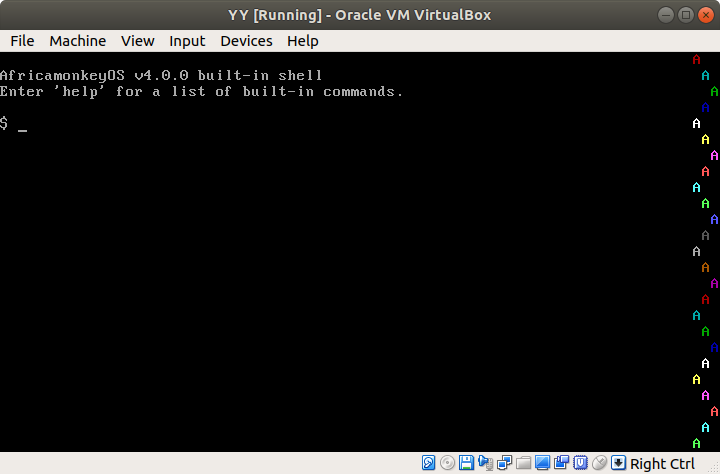
\includegraphics[scale=0.55]{pics/1.png}
\end{figure}

上图展示的是时钟中断功能。在屏幕右侧会有 'A' 字符不断反弹。

\begin{figure}[!hbp]
	\centering
	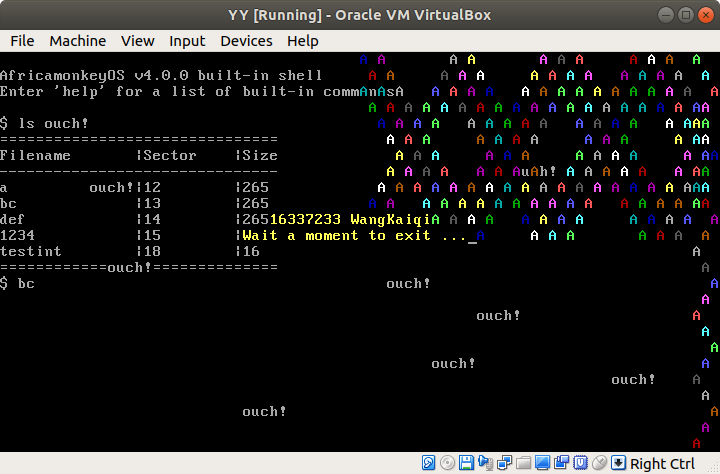
\includegraphics[scale=0.55]{pics/2.png}
\end{figure}

上图展示的是键盘中断功能。输入前 4 个用户程序(a, bc, def, 1234)即可响应键盘中断。键盘按下和弹起时,会在屏幕上\textbf{随机一个位置}显示 ouch! 。

\newpage

\begin{figure}[!hbp]
	\centering
	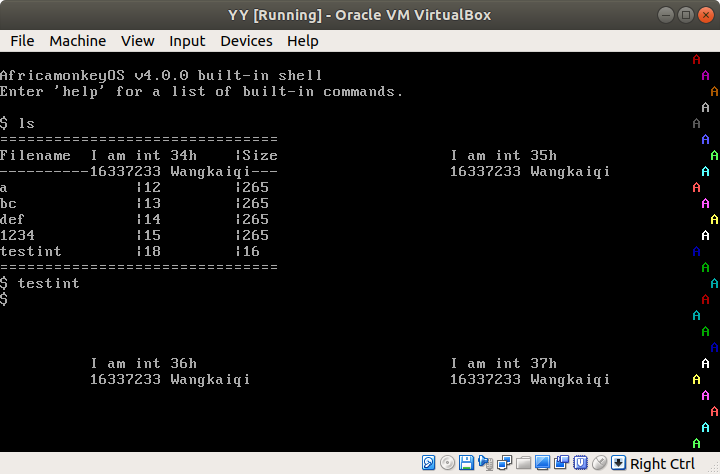
\includegraphics[scale=0.55]{pics/3.png}
\end{figure}

上图展示的是系统调用功能。输入第 5 个程序(testint)即可依次调用 int 34h, 35h, 36h, 37h 。每个程序分别在对应 1/4 位置显示相关信息。

\section{实验总结}

这次实验让我深入理解了中断服务程序的工作原理。中断响应后,先到内存指定位置找到中断向量表,然后跳转到中断服务程序。中断服务程序需先保存寄存器。中断服务程序完成后,需先还原寄存器,然后调用中断返回指令。所以在做实验的时候,就需要修改操作系统内核,使操作系统内核修改中断向量表,才能实现自定义中断服务程序。

\end{document}
















